\section{椭圆曲线上的点群}\label{sec:15-1}

椭圆曲线在数学的几个分支中都有出现。在这里,我们主要关注它们作为算术(对有理数的研究)这一分支的发展。我们的故事从丢潘图 (Diophantus) 开始,他是公元 3 世纪生活在亚历山大的希腊数学家。丢潘图对以下问题感兴趣:给定一个二元多项式方程 $f(x,y)=0$,找到满足该方程的有理点。所谓有理点指的是两个坐标都是有理数的点,比如 $({1}/{2},{1}/{3})$ 是一个有理点,但 $(1,\sqrt{2})$ 就不是。丢番图就这一问题写了一系列有影响的书,称为\emph{《算术》(Arithmetica)},其中有六卷有幸保存至今。14 个世纪后,费马 (Fermat) 在《算术》拉丁文译本的空白处写下了他著名的猜想。Bashmakova 的一本颇有见地的小册子用现代数学的语言描述了丢番图的思想。

《算术》的大部分内容都是在研究一元二次方程的整数解和有理解。然而,在少数地方,丢番图考虑了更高层次的问题。在第 4 卷的问题 24 中,椭圆曲线首次出现,它研究的是一个三次方程。该问题等价于以下问题:找到满足方程:
\begin{equation}\label{eq:15-1}
y^2=x^3-x+9
\end{equation}
的有理点 $(x,y)\in\mathbb{Q}^2$。图 \ref{fig:15-1} 展示了这条曲线在实数域上的分布情况。我们不知道是什么迫使丢番图提出这个问题,但可以想见,如果他知道他发明的方法在十几个世纪之后被广泛用于保护全世界数十亿人的互联网流量,他一定会倍感震惊。

我们很容易验证六个整数点 $(0,\pm3)$,$(1,\pm3)$,$(-1,\pm3)$ 都在式 \ref{eq:15-1} 的曲线上。但是,丢番图想在这条曲线上找到更多的有理点。

他开始从已有的六个点中派生出新的有理点。下面是一种方法,但与丢番图的做法稍有不同。令 $P:=(-1,-3)$,$Q:=(1,3)$,这两个点显然都满足式 \ref{eq:15-1}。让我们看一下经过 $P$ 和 $Q$ 的直线,如图 \ref{fig:15-1-b} 所示。我们很容易验证这条直线就是 $y=3x$,而且它必然与曲线 $y^2=x^3-x+9$ 恰好有三个交点。想要知道为什么,可以观察到,如果我们用 $3x$ 代换式 \ref{eq:15-1} 中的 $y$,就能够得到一个单变量的三次方程 $(3x)^2=x^3-x+9$。我们现在已经知道了这个三次方程的两个有理根,即$P$ 点对应的 $x_1=-1$ 和 $Q$ 点对应的 $x_2=1$。不难知道,有两个有理系数的三次方程在已有两个有理根的情况下,也一定能找到第三个有理根 $x_3$。在我们的例子中,这第三个有理根恰好是 $x_3=9$。设置 $y_3=3x_3$,我们就得到曲线 \ref{eq:15-1} 上的一个新点,即 $(9,27)$。我们暂且用 $-R$ 来表示这个点,原因我们将会马上说明。同时,我们也能立即得到另一个点 $(9,-27)$,我们将其记为 $R$。更一般地,对于曲线上的一个点 $T=(x,y)$,我们记 $-T:=(x,-y)$。

这种建立有理点的技术被称为\textbf{割弦法 (chord method)}。这种方法非常普适:给定曲线上两个不同的有理点 $U$ 和 $V$,其中 $U\neq-V$,我们就可以构造一条穿过这两点的直线,而这条直线必然与曲线交于第三个有理点 $-W$。例如,对上面的点 $P$ 和 $R$ 应用这种方法,我们就可以得到两个新的点 $(-56/25,3/125)$ 和 $(-56/25,-3/125)$。

几个世纪以来,割弦法被重新发现了好几次,但它最终被庞加莱 (Poincaré) 在代数曲线上的工作确定下来。庞加莱把从两个已知的有理点构建一个新的有理点的过程比作是一个群中的加法运算。具体来说,对于曲线上的不同点 $U$ 和 $V$,其中 $U\neq-V$,令 $-W$ 是曲线上的另一个点,该点与 $U$ 和 $V$ 共线,是直线与曲线的第三个交点。然后,庞加莱将 $U$ 与 $V$ 的加法表示为 $U\boxplus V$,有:
\begin{equation}\label{eq:15-2}
U\boxplus V=-W
\end{equation}
图 \ref{fig:15-1-b} 展示了在点 $P$ 和 $Q$ 上应用这一加法规则的结果。它们的和 $P\boxplus Q$ 就是点 $R=(9,27)$。使用式 \ref{eq:15-2} 的方法定义加法,当定义的方式比较妥当时,这个操作就具有结合性。回顾一下,结核性意味着 $(U\boxplus V)\boxplus W=U\boxplus(V\boxplus W)$。


\begin{figure}
  \centering
  \subfigure[曲线]{
    \begin{tikzpicture}

\begin{axis}[%
width=2.6in,
height=2.8in,
axis lines=middle,
axis line style={->},
tick style={color=black},
xtick=\empty,ytick=\empty,
xlabel=$x$,
ylabel=$y$,
xmin=-5,
xmax=20,
ymin=-30,
ymax=30
]

\addplot [forget plot]
  table[row sep=crcr]{%
-2.25	0\\
-2.24	0.023999999999938\\
-2.23	0.374743912558965\\
-2.22	0.528159066948584\\
-2.21	0.645088366039879\\
-2.2	0.742967024840266\\
-2.19	0.828577697020623\\
-2.18	0.90541040418144\\
-2.17	0.975544463363921\\
-2.16	1.04033840648127\\
-2.15	1.10073838853744\\
-2.14	1.15743509537252\\
-2.13	1.21095127895386\\
-2.12	1.2616940992174\\
-2.11	1.3099881678855\\
-2.1	1.35609734163887\\
-2.09	1.4002396223504\\
-2.08	1.44259765700628\\
-2.07	1.48332632957148\\
-2.06	1.52255837326521\\
-2.05	1.56040860033518\\
-2.04	1.59697714448266\\
-2.03	1.63235198410147\\
-2.02	1.66661093240144\\
-2.01	1.69982322610323\\
-2	1.73205080756888\\
-2	1.73205080756888\\
-1.9	2.01022386813011\\
-1.8	2.22890107452081\\
-1.7	2.40561842360753\\
-1.6	2.55029410068721\\
-1.5	2.66926956300783\\
-1.4	2.7669477768834\\
-1.3	2.84657689163669\\
-1.2	2.91067002595622\\
-1.1	2.96124973617559\\
-1	3\\
-0.9	3.02836589599077\\
-0.8	3.04762202380807\\
-0.7	3.05892137852544\\
-0.6	3.06333151976733\\
-0.5	3.06186217847897\\
-0.4	3.05548686791483\\
-0.3	3.0451600943136\\
-0.2	3.03183112986195\\
-0.0999999999999999	3.01645487285986\\
0	3\\
0.1	2.98345437370844\\
0.2	2.96782748824793\\
0.3	2.95414962383424\\
0.4	2.94346734311764\\
0.5	2.93683503111768\\
0.6	2.93530236943317\\
0.7	2.93989795741281\\
0.8	2.95160973029972\\
0.9	2.97136332345945\\
1	3\\
1.1	3.03825607873991\\
1.2	3.08674585931528\\
1.3	3.14594977709435\\
1.4	3.21620894843603\\
1.5	3.29772648956823\\
1.6	3.39057517244493\\
1.7	3.49471028842163\\
1.8	3.60998614955792\\
1.9	3.73617451412538\\
2	3.87298334620742\\
2.1	4.020074626173\\
2.2	4.17708032003216\\
2.3	4.34361600512752\\
2.4	4.51929197994553\\
2.5	4.70372193055669\\
2.6	4.89652938314476\\
2.7	5.09735225386671\\
2.8	5.3058458326642\\
2.9	5.52168452557732\\
3	5.74456264653803\\
3.1	5.9741945063749\\
3.2	6.21031400172326\\
3.3	6.45267386437592\\
3.4	6.70104469467262\\
3.5	6.95521387162178\\
3.6	7.21498440746756\\
3.7	7.48017379477242\\
3.8	7.75061287899222\\
3.9	8.02614477816093\\
4	8.30662386291807\\
4.1	8.59191480404688\\
4.2	8.88189169040019\\
4.3	9.17643721713389\\
4.4	9.47544194219985\\
4.5	9.77880360780397\\
4.6	10.0864265228078\\
4.7	10.3982210016906\\
4.8	10.7141028555824\\
4.9	11.0339929309385\\
5	11.3578166916005\\
5.1	11.6855038402287\\
5.2	12.0169879753622\\
5.3	12.352206280661\\
5.4	12.6910992431704\\
5.5	13.0336103977371\\
5.6	13.3796860949725\\
5.7	13.729275290415\\
5.8	14.082329352774\\
5.9	14.4388018893536\\
6	14.7986485869487\\
6.1	15.161827066683\\
6.2	15.5282967514148\\
6.3	15.8980187444851\\
6.4	16.2709557187032\\
6.5	16.6470718145865\\
6.6	17.0263325469697\\
6.7	17.4087047191915\\
6.8	17.7941563441485\\
6.9	18.1826565715794\\
7	18.5741756210067\\
7.1	18.9686847198218\\
7.2	19.3661560460511\\
7.3	19.7665626753869\\
7.4	20.1698785321082\\
7.5	20.5760783435523\\
7.6	20.9851375978334\\
7.7	21.397032504532\\
7.8	21.8117399581051\\
7.9	22.2292375037922\\
8	22.6495033058122\\
8.1	23.0725161176669\\
8.2	23.4982552543801\\
8.3	23.9267005665219\\
8.4	24.3578324158781\\
8.5	24.7916316526363\\
8.6	25.2280795939762\\
8.7	25.6671580039552\\
8.8	26.1088490745954\\
8.9	26.5531354080832\\
9	27\\
9.1	27.4494262235115\\
9.2	27.9013978144465\\
9.3	28.3558988572043\\
9.4	28.8129137714324\\
9.5	29.2724272994229\\
9.6	29.7344244941785\\
9.7	30.1988907081038\\
9.8	30.6658115822817\\
9.9	31.1351730362945\\
10	31.6069612585582\\
};
\addplot [forget plot]
  table[row sep=crcr]{%
-2.25	-0\\
-2.24	-0.023999999999938\\
-2.23	-0.374743912558965\\
-2.22	-0.528159066948584\\
-2.21	-0.645088366039879\\
-2.2	-0.742967024840266\\
-2.19	-0.828577697020623\\
-2.18	-0.90541040418144\\
-2.17	-0.975544463363921\\
-2.16	-1.04033840648127\\
-2.15	-1.10073838853744\\
-2.14	-1.15743509537252\\
-2.13	-1.21095127895386\\
-2.12	-1.2616940992174\\
-2.11	-1.3099881678855\\
-2.1	-1.35609734163887\\
-2.09	-1.4002396223504\\
-2.08	-1.44259765700628\\
-2.07	-1.48332632957148\\
-2.06	-1.52255837326521\\
-2.05	-1.56040860033518\\
-2.04	-1.59697714448266\\
-2.03	-1.63235198410147\\
-2.02	-1.66661093240144\\
-2.01	-1.69982322610323\\
-2	-1.73205080756888\\
-2	-1.73205080756888\\
-1.9	-2.01022386813011\\
-1.8	-2.22890107452081\\
-1.7	-2.40561842360753\\
-1.6	-2.55029410068721\\
-1.5	-2.66926956300783\\
-1.4	-2.7669477768834\\
-1.3	-2.84657689163669\\
-1.2	-2.91067002595622\\
-1.1	-2.96124973617559\\
-1	-3\\
-0.9	-3.02836589599077\\
-0.8	-3.04762202380807\\
-0.7	-3.05892137852544\\
-0.6	-3.06333151976733\\
-0.5	-3.06186217847897\\
-0.4	-3.05548686791483\\
-0.3	-3.0451600943136\\
-0.2	-3.03183112986195\\
-0.0999999999999999	-3.01645487285986\\
0	-3\\
0.1	-2.98345437370844\\
0.2	-2.96782748824793\\
0.3	-2.95414962383424\\
0.4	-2.94346734311764\\
0.5	-2.93683503111768\\
0.6	-2.93530236943317\\
0.7	-2.93989795741281\\
0.8	-2.95160973029972\\
0.9	-2.97136332345945\\
1	-3\\
1.1	-3.03825607873991\\
1.2	-3.08674585931528\\
1.3	-3.14594977709435\\
1.4	-3.21620894843603\\
1.5	-3.29772648956823\\
1.6	-3.39057517244493\\
1.7	-3.49471028842163\\
1.8	-3.60998614955792\\
1.9	-3.73617451412538\\
2	-3.87298334620742\\
2.1	-4.020074626173\\
2.2	-4.17708032003216\\
2.3	-4.34361600512752\\
2.4	-4.51929197994553\\
2.5	-4.70372193055669\\
2.6	-4.89652938314476\\
2.7	-5.09735225386671\\
2.8	-5.3058458326642\\
2.9	-5.52168452557732\\
3	-5.74456264653803\\
3.1	-5.9741945063749\\
3.2	-6.21031400172326\\
3.3	-6.45267386437592\\
3.4	-6.70104469467262\\
3.5	-6.95521387162178\\
3.6	-7.21498440746756\\
3.7	-7.48017379477242\\
3.8	-7.75061287899222\\
3.9	-8.02614477816093\\
4	-8.30662386291807\\
4.1	-8.59191480404688\\
4.2	-8.88189169040019\\
4.3	-9.17643721713389\\
4.4	-9.47544194219985\\
4.5	-9.77880360780397\\
4.6	-10.0864265228078\\
4.7	-10.3982210016906\\
4.8	-10.7141028555824\\
4.9	-11.0339929309385\\
5	-11.3578166916005\\
5.1	-11.6855038402287\\
5.2	-12.0169879753622\\
5.3	-12.352206280661\\
5.4	-12.6910992431704\\
5.5	-13.0336103977371\\
5.6	-13.3796860949725\\
5.7	-13.729275290415\\
5.8	-14.082329352774\\
5.9	-14.4388018893536\\
6	-14.7986485869487\\
6.1	-15.161827066683\\
6.2	-15.5282967514148\\
6.3	-15.8980187444851\\
6.4	-16.2709557187032\\
6.5	-16.6470718145865\\
6.6	-17.0263325469697\\
6.7	-17.4087047191915\\
6.8	-17.7941563441485\\
6.9	-18.1826565715794\\
7	-18.5741756210067\\
7.1	-18.9686847198218\\
7.2	-19.3661560460511\\
7.3	-19.7665626753869\\
7.4	-20.1698785321082\\
7.5	-20.5760783435523\\
7.6	-20.9851375978334\\
7.7	-21.397032504532\\
7.8	-21.8117399581051\\
7.9	-22.2292375037922\\
8	-22.6495033058122\\
8.1	-23.0725161176669\\
8.2	-23.4982552543801\\
8.3	-23.9267005665219\\
8.4	-24.3578324158781\\
8.5	-24.7916316526363\\
8.6	-25.2280795939762\\
8.7	-25.6671580039552\\
8.8	-26.1088490745954\\
8.9	-26.5531354080832\\
9	-27\\
9.1	-27.4494262235115\\
9.2	-27.9013978144465\\
9.3	-28.3558988572043\\
9.4	-28.8129137714324\\
9.5	-29.2724272994229\\
9.6	-29.7344244941785\\
9.7	-30.1988907081038\\
9.8	-30.6658115822817\\
9.9	-31.1351730362945\\
10	-31.6069612585582\\
};
\end{axis}
\end{tikzpicture}%
    \label{fig:15-1-a}
  }
  \quad\quad\quad\quad
  \subfigure[添加点 $P=(-1,-3)$ 和点 $Q=(1,3)$]{
    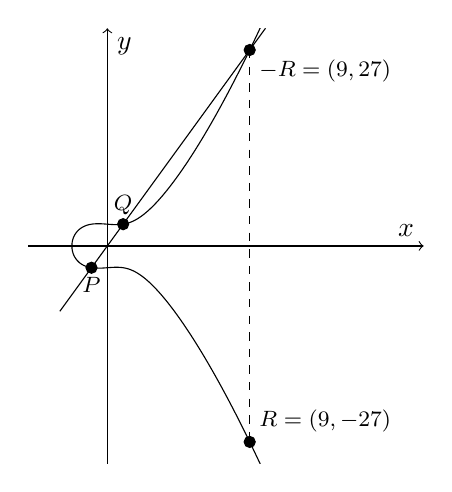
\begin{tikzpicture}

\begin{axis}[%
width=2.6in,
height=2.8in,
axis lines=middle,
axis line style={->},
tick style={color=black},
xtick=\empty,ytick=\empty,
xlabel=$x$,
ylabel=$y$,
xmin=-5,
xmax=20,
ymin=-30,
ymax=30
]

\addplot[
domain=-3:10, 
samples=100] {
3 * x
};

\addplot [forget plot]
  table[row sep=crcr]{%
-2.25	0\\
-2.24	0.023999999999938\\
-2.23	0.374743912558965\\
-2.22	0.528159066948584\\
-2.21	0.645088366039879\\
-2.2	0.742967024840266\\
-2.19	0.828577697020623\\
-2.18	0.90541040418144\\
-2.17	0.975544463363921\\
-2.16	1.04033840648127\\
-2.15	1.10073838853744\\
-2.14	1.15743509537252\\
-2.13	1.21095127895386\\
-2.12	1.2616940992174\\
-2.11	1.3099881678855\\
-2.1	1.35609734163887\\
-2.09	1.4002396223504\\
-2.08	1.44259765700628\\
-2.07	1.48332632957148\\
-2.06	1.52255837326521\\
-2.05	1.56040860033518\\
-2.04	1.59697714448266\\
-2.03	1.63235198410147\\
-2.02	1.66661093240144\\
-2.01	1.69982322610323\\
-2	1.73205080756888\\
-2	1.73205080756888\\
-1.9	2.01022386813011\\
-1.8	2.22890107452081\\
-1.7	2.40561842360753\\
-1.6	2.55029410068721\\
-1.5	2.66926956300783\\
-1.4	2.7669477768834\\
-1.3	2.84657689163669\\
-1.2	2.91067002595622\\
-1.1	2.96124973617559\\
-1	3\\
-0.9	3.02836589599077\\
-0.8	3.04762202380807\\
-0.7	3.05892137852544\\
-0.6	3.06333151976733\\
-0.5	3.06186217847897\\
-0.4	3.05548686791483\\
-0.3	3.0451600943136\\
-0.2	3.03183112986195\\
-0.0999999999999999	3.01645487285986\\
0	3\\
0.1	2.98345437370844\\
0.2	2.96782748824793\\
0.3	2.95414962383424\\
0.4	2.94346734311764\\
0.5	2.93683503111768\\
0.6	2.93530236943317\\
0.7	2.93989795741281\\
0.8	2.95160973029972\\
0.9	2.97136332345945\\
1	3\\
1.1	3.03825607873991\\
1.2	3.08674585931528\\
1.3	3.14594977709435\\
1.4	3.21620894843603\\
1.5	3.29772648956823\\
1.6	3.39057517244493\\
1.7	3.49471028842163\\
1.8	3.60998614955792\\
1.9	3.73617451412538\\
2	3.87298334620742\\
2.1	4.020074626173\\
2.2	4.17708032003216\\
2.3	4.34361600512752\\
2.4	4.51929197994553\\
2.5	4.70372193055669\\
2.6	4.89652938314476\\
2.7	5.09735225386671\\
2.8	5.3058458326642\\
2.9	5.52168452557732\\
3	5.74456264653803\\
3.1	5.9741945063749\\
3.2	6.21031400172326\\
3.3	6.45267386437592\\
3.4	6.70104469467262\\
3.5	6.95521387162178\\
3.6	7.21498440746756\\
3.7	7.48017379477242\\
3.8	7.75061287899222\\
3.9	8.02614477816093\\
4	8.30662386291807\\
4.1	8.59191480404688\\
4.2	8.88189169040019\\
4.3	9.17643721713389\\
4.4	9.47544194219985\\
4.5	9.77880360780397\\
4.6	10.0864265228078\\
4.7	10.3982210016906\\
4.8	10.7141028555824\\
4.9	11.0339929309385\\
5	11.3578166916005\\
5.1	11.6855038402287\\
5.2	12.0169879753622\\
5.3	12.352206280661\\
5.4	12.6910992431704\\
5.5	13.0336103977371\\
5.6	13.3796860949725\\
5.7	13.729275290415\\
5.8	14.082329352774\\
5.9	14.4388018893536\\
6	14.7986485869487\\
6.1	15.161827066683\\
6.2	15.5282967514148\\
6.3	15.8980187444851\\
6.4	16.2709557187032\\
6.5	16.6470718145865\\
6.6	17.0263325469697\\
6.7	17.4087047191915\\
6.8	17.7941563441485\\
6.9	18.1826565715794\\
7	18.5741756210067\\
7.1	18.9686847198218\\
7.2	19.3661560460511\\
7.3	19.7665626753869\\
7.4	20.1698785321082\\
7.5	20.5760783435523\\
7.6	20.9851375978334\\
7.7	21.397032504532\\
7.8	21.8117399581051\\
7.9	22.2292375037922\\
8	22.6495033058122\\
8.1	23.0725161176669\\
8.2	23.4982552543801\\
8.3	23.9267005665219\\
8.4	24.3578324158781\\
8.5	24.7916316526363\\
8.6	25.2280795939762\\
8.7	25.6671580039552\\
8.8	26.1088490745954\\
8.9	26.5531354080832\\
9	27\\
9.1	27.4494262235115\\
9.2	27.9013978144465\\
9.3	28.3558988572043\\
9.4	28.8129137714324\\
9.5	29.2724272994229\\
9.6	29.7344244941785\\
9.7	30.1988907081038\\
9.8	30.6658115822817\\
9.9	31.1351730362945\\
10	31.6069612585582\\
};
\addplot [forget plot]
  table[row sep=crcr]{%
-2.25	-0\\
-2.24	-0.023999999999938\\
-2.23	-0.374743912558965\\
-2.22	-0.528159066948584\\
-2.21	-0.645088366039879\\
-2.2	-0.742967024840266\\
-2.19	-0.828577697020623\\
-2.18	-0.90541040418144\\
-2.17	-0.975544463363921\\
-2.16	-1.04033840648127\\
-2.15	-1.10073838853744\\
-2.14	-1.15743509537252\\
-2.13	-1.21095127895386\\
-2.12	-1.2616940992174\\
-2.11	-1.3099881678855\\
-2.1	-1.35609734163887\\
-2.09	-1.4002396223504\\
-2.08	-1.44259765700628\\
-2.07	-1.48332632957148\\
-2.06	-1.52255837326521\\
-2.05	-1.56040860033518\\
-2.04	-1.59697714448266\\
-2.03	-1.63235198410147\\
-2.02	-1.66661093240144\\
-2.01	-1.69982322610323\\
-2	-1.73205080756888\\
-2	-1.73205080756888\\
-1.9	-2.01022386813011\\
-1.8	-2.22890107452081\\
-1.7	-2.40561842360753\\
-1.6	-2.55029410068721\\
-1.5	-2.66926956300783\\
-1.4	-2.7669477768834\\
-1.3	-2.84657689163669\\
-1.2	-2.91067002595622\\
-1.1	-2.96124973617559\\
-1	-3\\
-0.9	-3.02836589599077\\
-0.8	-3.04762202380807\\
-0.7	-3.05892137852544\\
-0.6	-3.06333151976733\\
-0.5	-3.06186217847897\\
-0.4	-3.05548686791483\\
-0.3	-3.0451600943136\\
-0.2	-3.03183112986195\\
-0.0999999999999999	-3.01645487285986\\
0	-3\\
0.1	-2.98345437370844\\
0.2	-2.96782748824793\\
0.3	-2.95414962383424\\
0.4	-2.94346734311764\\
0.5	-2.93683503111768\\
0.6	-2.93530236943317\\
0.7	-2.93989795741281\\
0.8	-2.95160973029972\\
0.9	-2.97136332345945\\
1	-3\\
1.1	-3.03825607873991\\
1.2	-3.08674585931528\\
1.3	-3.14594977709435\\
1.4	-3.21620894843603\\
1.5	-3.29772648956823\\
1.6	-3.39057517244493\\
1.7	-3.49471028842163\\
1.8	-3.60998614955792\\
1.9	-3.73617451412538\\
2	-3.87298334620742\\
2.1	-4.020074626173\\
2.2	-4.17708032003216\\
2.3	-4.34361600512752\\
2.4	-4.51929197994553\\
2.5	-4.70372193055669\\
2.6	-4.89652938314476\\
2.7	-5.09735225386671\\
2.8	-5.3058458326642\\
2.9	-5.52168452557732\\
3	-5.74456264653803\\
3.1	-5.9741945063749\\
3.2	-6.21031400172326\\
3.3	-6.45267386437592\\
3.4	-6.70104469467262\\
3.5	-6.95521387162178\\
3.6	-7.21498440746756\\
3.7	-7.48017379477242\\
3.8	-7.75061287899222\\
3.9	-8.02614477816093\\
4	-8.30662386291807\\
4.1	-8.59191480404688\\
4.2	-8.88189169040019\\
4.3	-9.17643721713389\\
4.4	-9.47544194219985\\
4.5	-9.77880360780397\\
4.6	-10.0864265228078\\
4.7	-10.3982210016906\\
4.8	-10.7141028555824\\
4.9	-11.0339929309385\\
5	-11.3578166916005\\
5.1	-11.6855038402287\\
5.2	-12.0169879753622\\
5.3	-12.352206280661\\
5.4	-12.6910992431704\\
5.5	-13.0336103977371\\
5.6	-13.3796860949725\\
5.7	-13.729275290415\\
5.8	-14.082329352774\\
5.9	-14.4388018893536\\
6	-14.7986485869487\\
6.1	-15.161827066683\\
6.2	-15.5282967514148\\
6.3	-15.8980187444851\\
6.4	-16.2709557187032\\
6.5	-16.6470718145865\\
6.6	-17.0263325469697\\
6.7	-17.4087047191915\\
6.8	-17.7941563441485\\
6.9	-18.1826565715794\\
7	-18.5741756210067\\
7.1	-18.9686847198218\\
7.2	-19.3661560460511\\
7.3	-19.7665626753869\\
7.4	-20.1698785321082\\
7.5	-20.5760783435523\\
7.6	-20.9851375978334\\
7.7	-21.397032504532\\
7.8	-21.8117399581051\\
7.9	-22.2292375037922\\
8	-22.6495033058122\\
8.1	-23.0725161176669\\
8.2	-23.4982552543801\\
8.3	-23.9267005665219\\
8.4	-24.3578324158781\\
8.5	-24.7916316526363\\
8.6	-25.2280795939762\\
8.7	-25.6671580039552\\
8.8	-26.1088490745954\\
8.9	-26.5531354080832\\
9	-27\\
9.1	-27.4494262235115\\
9.2	-27.9013978144465\\
9.3	-28.3558988572043\\
9.4	-28.8129137714324\\
9.5	-29.2724272994229\\
9.6	-29.7344244941785\\
9.7	-30.1988907081038\\
9.8	-30.6658115822817\\
9.9	-31.1351730362945\\
10	-31.6069612585582\\
};

\addplot [
only marks
] coordinates {
(-1,-3)
} node [pos=0,anchor=north] {\footnotesize $P$};
    
\addplot [
only marks
] coordinates {
(1,3)
} node [pos=0,anchor=south] {\footnotesize $Q$};

\addplot [
only marks
] coordinates {
(9,27)
} node [pos=0,anchor=north west] {\footnotesize $-R=(9,27)$};

\addplot [
only marks
] coordinates {
(9,-27)
} node [pos=0,anchor=south west] {\footnotesize $R=(9,-27)$};

\addplot[color=black,dashed]
coordinates {
(9,27)
(9,-27)
};
\end{axis}
\end{tikzpicture}%
    \label{fig:15-1-b}
  }
  \caption{实数域上的曲线 $y^2=x^3-x+9$}
  \label{fig:15-1}
\end{figure}

我们将在下一节展示如何加强这个加法规则,使得曲线上的点集能够构成一个群。数论中一些最优雅的结论,以及一些深刻的开放性问题,都来自于试图理解椭圆曲线上的有理点群的特性。

我们再说回丢番图,他在式 \ref{eq:15-1} 上寻找有理点的方法是我们刚才介绍的方法的一个变体。丢番图没有选择过两个不同的点的直线,而是选择了在其中一个已知点上作一条该曲线的切线。假设我们在点 $P=(-1,-3)$ 上作一条曲线的切线。和之前一样,不难证明,在有理系数的三次曲线上,如果 $(x_1,y_1)$ 是一个有理点,且 $y_1\neq0$,那么曲线在 $(x_1,y_1)$ 处的切线一定与曲线相交于另一个点 $T$,且 $T$ 也必然是一个有理点。在我们的例子中,曲线在 $P=(-1,-3)$ 处的切线是 $y=-{1/3}x-{10/3}$,该直线与曲线的另一个交点是 $({19/9},-{109/27})$,该点确实是一个有理点。这种方法被称为\textbf{切线法 (tangent method)},它是在 $y_1\neq0$时从一个给定的有理点 $(x_1,y_1)$ 建立一个新有理点的另一种方法。正如我们将看到的,它相当于将点 $P$ 与自己相加,即计算 $P\boxplus P$。